%-----------------------------------------------------------------------------%
\chapter{LANDASAN TEORI}
%-----------------------------------------------------------------------------%

%
\vspace{4.5pt}

\section{Tinjauan Pustaka}
\indent
Tinjauan pustaka merupakan bagian yang menjelaskan semua dasar teori yang dibutuhkan untuk melakukan penelitian ini.

\subsection{Pemrosesan Bahasa Alami}
\indent
Pemrosesan Bahasa Alami atau yang biasa disebut dengan singkatan PBA atau NLP adalah cara bagi komputer untuk menganalisa, memahami, dan memperoleh makna dari bahasa manusia dengan cara yang cerdas dan berguna. Interaksi manusia komputer ini memungkinkan aplikasi dunia nyata seperti {\itshape automatic text summarization}, {\itshape sentiment analysis}, {\itshape topic extraction}, {\itshape named entity recognition}, {\itshape parts-of-speech tagging}, {\itshape relationship extraction}, {\itshape stemming}, dll [5].

\indent 
NLP biasanya digunakan untuk {\itshape information retrieval}, {\itshape text mining}, {\itshape machine translation}, dan {\itshape automated question answering}. Jika dikaitkan dengan permasalahan pada penelitian ini, {\itshape text categorization} merupakan salah satu bagian terpenting dalam kasus {\itshape information retrieval} untuk meningkatkan akurasi informasi serta meningkatkan kepuasan pengguna terhadap informasi yang didapat [6].

\subsection{Klasifikasi Teks}
\indent
Klasifikasi Teks atau Kategorisasi Teks merupakan salah satu masalah pada {\itshape machine learning} yang bertujuan untuk mengelompokkan sekumpulan dokumen ke dalam kelompok tertentu. Masukan pada klasifikasi teks adalah berupa dokumen-dokumen yang telah diberi label. Label yang terdapat pada setiap dokumen dapat berjumlah 1 atau lebih, karena setiap dokumen pasti memiliki lebih dari 1 kategori.

\indent
Dengan menggunakan {\itshape machine learning}, masukan yang telah disebutkan di atas akan digunakan sistem untuk belajar agar dapat mengenali pola dari dokumen yang diberikan, dimana pola yang didapat akan menghasilkan suatu model. Model ini kemudian akan digunakan sistem untuk menghasilkan sebuah keluaran berupa kategori atau label. Contoh sederhana untuk klasifikasi teks adalah {\itshape movie genre classification}, dimana masukan kasus ini dapat berupa sinopsis dari setiap film dan label yang akan digunakan untuk setiap film adalah {\itshape “thriller”, “romantic”, “terror”, “horror”}, dll.

\subsection{Pembelajaran Mesin}
\indent
Pembelajaran Mesin ({\itshape machine learning}) merupakan cara bagi komputer untuk belajar agar dapat berpikir dan mengambil keputusan seperti manusia. Masukan yang dibutuhkan oleh komputer adalah data yang memiliki fitur yang sesuai dengan masalah yang ingin diselesaikan. Sebagai contoh jika masalah yang dihadapi merupakan kategorisasi buku maka data yang dibutuhkan dapat berupa buku-buku dengan sinopsis sebagai fiturnya. Data ini akan digunakan komputer sebagai sumber pembelajaran dalam mengambil keputusan.

\indent
Pembelajaran mesin pada dunia nyata dapat diimplementasikan untuk {\itshape text classification}, {\itshape fraud detection}, {\itshape pattern and image recognition}, {\itshape new pricing models}, dll. Secara mendasar teknik pada pembelajaran mesin dapat diklasifikasikan menjadi 3 kelompok. Kelompok ini di antaranya adalah {\itshape supervised learning}, {\itshape unsupervised learning}, dan {\itshape reinforcement learning}. Pada penelitian ini, teknik pembelajaran mesin yang akan digunakan adalah {\itshape supervised learning} dan masalah yang akan diteliti adalah mengenai klasifikasi teks. Berikut merupakan beberapa terminologi yang terdapat dalam pembelajaran mesin [1].

\begin{enumerate}[nolistsep,leftmargin=0.5cm]
\item
Data Belajar, merupakan data yang digunakan selama proses pembelajaran untuk menghasilkan data model. Data pada data belajar harus berisi informasi yang sesuai.
\item
Data Model, merupakan data yang didapat dari proses belajar yang berfungsi untuk basis dalam pengambilan keputusan.
\item
Proses Belajar, merupakan proses mengolah data belajar agar dapat menghasilkan suatu model.
\item
Data Uji, merupakan data yang digunakan ketika melakukan pengujian. Proses pengujian akan menggunakan model yang didapat dari proses belajar untuk menentukan kategori dari data yang ingin diuji.
\item
Fitur ({\itshape Feature}), merupakan karakteristik unik yang dimiliki sebuah objek.
\item
Seleksi fitur ({\itshape Feature Selection}) merupakan proses memilih {\itshape subset} dari fitur yang relevan untuk digunakan dalam pembangunan model.
\item
{\itshape Classification}, merupakan proses mengambil beberapa jenis masukan dan menetapkan label pada masukan tersebut.
\end{enumerate}

\subsubsection{Mesin Pembelajaran Terarah ({\itshape Supervised Learning})}
\indent
Mesin Pembelajaran Terarah secara mendasar merupakan salah satu bagian dari teknik pembelajaran mesin untuk membuat komputer agar dapat berpikir seperti manusia. Mesin pembelajaran terarah melakukan pembelajaran terhadap mesin dengan bantuan manusia untuk menentukan suatu pilihan. Masukan dari teknik mesin pembelajaran terarah harus memiliki label pada setiap data belajar yang akan digunakan. Label yang ditetapkan dapat berupa {\itshape single label} (1 label) maupun {\itshape multi label} (lebih dari 1 label). Berikut merupakan langkah-langkah dalam memecahkan masalah pada mesin pembelajaran terarah.

\begin{enumerate}[nolistsep,leftmargin=0.5cm]
\item
Menentukan jenis data yang akan digunakan sebagai data belajar. Dalam kasus kategorisasi teks, contoh data yang dapat digunakan adalah abstraksi jurnal penelitian, isi berita, atau sinopsis film.
\item
Kumpulkan data belajar, dimana data belajar harus merepresentasikan kasus pada dunia nyata.
\item
Menentukan masukan fitur yang akan digunakan dalam proses belajar. Jumlah fitur dapat mempengaruhi tingkat akurasi yang dihasilkan. Jumlah fitur tidak boleh terlalu besar, namun harus berisi cukup informasi untuk menghasilkan keluaran yang akurat.
\item
Menentukan algoritma pembelajaran yang sesuai. Sebagai contoh, algoritma yang dapat digunakan untuk kategorisasi adalah {\itshape Labeled Latent Dirichlet Allocation}, {\itshape Support Vector Machine}, atau {\itshape Naïve Bayes}.
\item
Melakukan proses pembelajaran terhadap data belajar menggunakan algoritma {\itshape supervised learning}. Beberapa algoritma {\itshape supervised learning} mengharuskan pengguna untuk menentukan parameter tertentu. Parameter ini digunakan untuk mengoptimalkan kinerja dari data belajar.
\item
Mengevaluasi akurasi dengan cara menguji hasil data belajar yang telah dipelajari dengan data uji.
\end{enumerate}

\subsection{{\itshape Text Pre-Processing}}
\indent
{\itshape Pre-processing} adalah proses normalisasi teks sehingga informasi yang dimuat merupakan bagian yang padat dan ringkas namun tetap merepresentasikan informasi yang termuat di dalamnya. Tahapan untuk melakukan {\itshape pre-processing} ini adalah {\itshape case folding}, {\itshape filtering}, {\itshape tokenizing}, {\itshape stopword removing}, dan {\itshape stemming} [7].

\begin{enumerate}[nolistsep,leftmargin=0.5cm]
\item
{\itshape Case Folding}\\
{\itshape Case Folding} merupakan proses mengubah bentuk huruf pada setiap kata menjadi bentuk huruf kecil. Tahap ini berfungsi untuk mengurangi jumlah fitur kata yang digunakan.
\item
{\itshape Filtering}\\
{\itshape Filtering} merupakan proses untuk menghapus tanda baca dan kata penghubung pada setiap kalimat. Tahap ini berfungsi untuk mempermudah pembacaan setiap kata untuk proses selanjutnya.
\item
{\itshape Tokenizing}\\
{\itshape Tokenizing} merupakan proses pemotongan dari bentuk kalimat menjadi kumpulan kata-kata yang disebut sebagai {\itshape token}. {\itshape Token} akan digunakan sebagai representasi data pada tiap baris yang ada di matriks probabilitas. Teknik {\itshape tokenizing} untuk mengubah suatu kalimat menjadi sebuah {\itshape token} adalah {\itshape word tokenizing}.  Sebagai contoh bila terdapat dokumen berisi kalimat sebagai berikut.

\begin{center}
“{\itshape I want to eat rice}”
\end{center}

Maka hasil {\itshape word tokenizing} dari kalimat tersebut akan menjadi seperti di bawah ini.

\begin{center}
{\itshape [I] [want] [to] [eat] [rice]}
\end{center}

\item
{\itshape Stopword Removing}\\
{\itshape Stopword Removing} merupakan proses penghapusan kata-kata yang tidak mewakili makna dari suatu kalimat. Salah satu sumber untuk mendapatkan daftar {\itshape stopword} adalah pada website www.ranks.nl. Contoh {\itshape stopword} yang didapat dari sumber tersebut di antaranya seperti {\itshape “am, is, are, and, in, none, however, the, etc”}.

\item
{\itshape Stemming}\\
{\itshape Stemming} merupakan proses untuk merubah sebuah kata menjadi kata dasar sesuai dengan pembentuk kata tersebut. Caranya adalah dengan menghilangkan imbuhan yang melekat pada kata, sehingga hasilnya adalah kata dasarnya. Dalam Bahasa Inggris, proses {\itshape stemming} bisa mengikutsertakan pengembalian bentuk {\itshape tense} dari kata kerja bentuk ke-2 atau ke-3 menjadi kata kerja bentuk ke-1. Sebagai contoh dalam kamus Bahasa Inggirs kata {\itshape “categorization”} berasal dari kata {\itshape “categorize”}.
\end{enumerate}

\subsection{{\itshape Regular Expression}}
\indent
{\itshape Regular Expression} ({\itshape regex}) merupakan teks khusus yang digunakan sebagai pola untuk mencocokan sekumpulan {\itshape string}. {\itshape Regular expression} mulai muncul pada tahun 1940-an sebagai cara untuk menggambarkan bahasa-bahasa pada umumnya, namun {\itshape regular expression} benar-benar muncul pada dunia {\itshape programming} sekitar tahun 1970-an. {\itshape Regular expression} pertama kali digunakan pada QED {\itshape text editor} oleh Ken Thompson. Sebagai contoh {\itshape regex} untuk mencocokkan angka antara 0 sampai 9 adalah seperti di bawah ini [8].

\begin{center}
\^{}($\backslash$($\backslash$d\{3\}$\backslash$)$\mid$\^{}$\backslash$d\{3\}$[$.-$]$?)?$\backslash$d\{3\}$[$.-$]$?$\backslash$d\{4\}$\backslash$\$
%^(\(\d{3}\)|^\d{3}[.-]?)?\d{3}[.-]?\d{4}\$
\end{center}

\subsection{Algoritma {\itshape Snowball Stememer}}
\indent
{\itshape Snowball Stemmer} merupakan metode {\itshape stemming} yang dikembangkan dari {\itshape Porter Stemmer}. Algoritma {\itshape Porter Stemmer} mulai diperkenalkan pada tahun 1980. Algoritma ini merupakan salah satu {\itshape stemmer} yang umum digunakan karena menghasilkan hasil {\itshape stemming} yang baik dibanding {\itshape stemmer} yang lainnya, selain itu juga nilai {\itshape error} yang dihasilkan {\itshape Porter Stemmer} dapat dikatakan kecil [9]. Untuk dapat lebih memahami algoritma dari {\itshape Porter Stemmer}, berikut merupakan cara kerja penggunaan algoritma {\itshape Snowball Stemmer} ({\itshape Porter Stemmer} yang dikembangkan).

\begin{enumerate}[nolistsep,leftmargin=0.5cm]
\item
Menghapus akhiran ‘, ‘s, dan ‘s’ jika ditemukan.
\item
Menangani {\itshape plural} dan {\itshape past participle}. Mencari akhiran pada Tabel 2.1 dan mengganti akhiran tersebut sesuai dengan tugasnya masing-masing.

\begin{table}[H]
\small
\centering
\caption{Langkah ke-2 {\itshape Snowball Stemmer}}
\begin{adjustbox}{width=1\textwidth}
\begin{tabular}{| p {3cm} | p {6cm} | p {5cm}|}
\hline
{\bfseries Akhiran} & {\bfseries Hasil ({\itshape Replace})} & {\bfseries Contoh} \\ 
\hline
SSES & SS & Caresses $\rightarrow$ Caress \\ 
\hline
\multirow{2}{*}{IES} & I (Jika lebih dari 1 huruf) & Ponies $\rightarrow$ Poni \\ 
\cline{2-3} & IE & Ties $\rightarrow$ tie \\
\hline
SS & SS & Caress $\rightarrow$ Caress \\
\hline
S & & Cats $\rightarrow$ Cat \\
\hline
\multirow{2}{*}{EED} & EE (Jika lebih dari 1 huruf) & Agreed $\rightarrow$ Agree \\
\cline{2-3} & & Feed $\rightarrow$ Feed \\
\hline
\end{tabular}
\end{adjustbox}
\end{table}

\begin{table}[H]
\small
\centering
\caption{Langkah ke-2 {\itshape Snowball Stemmer}}
\begin{adjustbox}{width=1\textwidth}
\begin{tabular}{| p {3cm} | p {6cm} | p {5cm}|}
\hline
ED, ING & & Motoring $\rightarrow$ Motor \\
\hline
Y & I (Jika didahului oleh konsonan yang bukan huruf pertama dari kata tersebut) & Cry $\rightarrow$ Cri \\
\hline
\end{tabular}
\end{adjustbox}
\end{table}

\noindent
Terdapat penanganan khusus untuk akhiran ED dan ING setelah dilakukan penghapusan. Tabel 2.2 merupakan penanganan untuk akhiran ED dan ING.

\begin{table}[H]
\small
\centering
\caption{Kondisi ED dan ING Pada {\itshape Snowball Stemmer}}
\begin{adjustbox}{width=1\textwidth}
\begin{tabular}{| p {5cm} | p {4cm} | p {5cm}|}
\hline
{\bfseries Kondisi} & {\bfseries Hasil ({\itshape Replace})} & {\bfseries Contoh} \\ 
\hline
Di akhiri at, bl, iz & e & Luxuriat $\rightarrow$ Luxuriate \\ 
\hline
Di akhiri 2 huruf yang sama &  & Hopp $\rightarrow$ Hop \\
\hline
Terdiri dari 3 huruf (short) & e & Hop $\rightarrow$ Hope \\
\hline
\end{tabular}
\end{adjustbox}
\end{table}

\item 
Mencari akhiran pada Tabel 2.3 dan mengganti akhiran tersebut sesuai dengan tugasnya masing-masing.

\begin{table}[H]
\small
\caption{ Langkah ke-3 {\itshape Snowball Stemmer}}
\begin{adjustbox}{width=1\textwidth}
\begin{tabular}{| p {3.5cm} | p {3.5cm} | p {7cm}|}
\hline
{\bfseries Akhiran} & {\bfseries Hasil ({\itshape Replace})} & {\bfseries Contoh} \\ 
\hline
ATIONAL & ATE & Relational $\rightarrow$ Relate \\
\hline
TIONAL & TION & Conditional $\rightarrow$ Condition \\
\hline
ENCI & ENCE & Valenci $\rightarrow$ Valence \\
\hline
ANCI & ANCE & Hesitanci $\rightarrow$ Hesitance \\
\hline
IZER & IZE & Digitizer $\rightarrow$ Digitize \\
\hline
ABLI & ABLE & Conformabli $\rightarrow$ Conformable \\
\hline
ALLI & AL & Radicalli $\rightarrow$ Radical \\
\hline
ENTLI & ENT & Differentli $\rightarrow$ Different \\
\hline
ELI & E & Vileli $\rightarrow$ Vile \\
\hline
OUSLI & OUS & Analogousli $\rightarrow$ Analogous \\
\hline
IZATION & IZE & Vietnamization $\rightarrow$ Vietnamize \\
\hline
ATION & ATE & Predication $\rightarrow$ Predicate \\
\hline
\end{tabular}
\end{adjustbox}
\end{table}

\begin{table}[H]
\small
\begin{adjustbox}{width=1\textwidth}
\begin{tabular}{| p {3.5cm} | p {3.5cm} | p {7cm}|}
\hline
ATOR & ATE & Operator $\rightarrow$ Operate \\
\hline
ALISM & AL & Feudalism $\rightarrow$ Feudal \\
\hline
IVENESS & IVE & Decisiveness $\rightarrow$ Decisive \\
\hline
FULNESS & FUL & Hopefulness $\rightarrow$ Hopeful \\
\hline
OUSNESS & OUS & Callousness $\rightarrow$ Callous \\
\hline
ALITI & AL & Formaliti $\rightarrow$ Formal \\
\hline
IVITI & IVE & Sensitiviti $\rightarrow$ Sensitive \\
\hline
BILITI & BLE & Sensibiliti $\rightarrow$ Sensible \\
\hline
\end{tabular}
\end{adjustbox}
\end{table}

\item 
Mencari akhiran pada Tabel 2.4 dan mengganti akhiran tersebut sesuai dengan tugasnya masing-masing.

\begin{table}[H]
\small
\caption{Langkah ke-4 {\itshape Snowball Stemmer}}
\begin{adjustbox}{width=1\textwidth}
\begin{tabular}{| p {3.5cm} | p {3.5cm} | p {7cm}|}
\hline
{\bfseries Akhiran} & {\bfseries Hasil ({\itshape Replace})} & {\bfseries Contoh} \\ 
\hline
ICATE & IC & Triplicate $\rightarrow$ triplic \\
\hline
ATIVE &  & Formative $\rightarrow$ form \\
\hline
ALIZE & AL & Formalize $\rightarrow$ formal \\
\hline
ICITI & IC & Electriciti $\rightarrow$ electric \\
\hline
ICAL & IC & Electrical $\rightarrow$ electric \\
\hline
FUL &  & Hopeful $\rightarrow$ hope \\
\hline
NESS &  & Goodness $\rightarrow$ good \\
\hline
\end{tabular}
\end{adjustbox}
\end{table}

\item
Mencari akhiran pada Tabel 2.5 dan mengganti akhiran tersebut sesuai dengan tugasnya masing-masing. Langkah ini merupakan langkah terakhir untuk menghapus akhiran dalam Bahasa Inggris.

\begin{table}[H]
\small
\caption{Langkah ke-5 {\itshape Snowball Stemmer}}
\begin{adjustbox}{width=1\textwidth}
\begin{tabular}{| p {3.5cm} | p {3.5cm} | p {7cm}|}
\hline
{\bfseries Akhiran} & {\bfseries Hasil ({\itshape Replace})} & {\bfseries Contoh} \\ 
\hline
AL & & Revival $\rightarrow$ Reviv \\
\hline
ANCE & & Allowance $\rightarrow$ Allow \\
\hline
ENCE & & Inference $\rightarrow$ Infer \\
\hline
\end{tabular}
\end{adjustbox}
\end{table}

\begin{table}[H]
\small
\begin{adjustbox}{width=1\textwidth}
\begin{tabular}{| p {3.5cm} | p {3.5cm} | p {7cm}|}
\hline
ER & & Airliner $\rightarrow$ Airlin \\
\hline
IC & & Gyroscopic $\rightarrow$ Gyroscop \\
\hline
ABLE & & Adjustable $\rightarrow$ Adjust \\
\hline
IBLE & & Defensible $\rightarrow$ Defens \\
\hline
ANT & & Irritant $\rightarrow$ Irrit \\
\hline
EMENT & & Replacement $\rightarrow$ Replac \\
\hline
MENT & & Adjustment $\rightarrow$ Adjust \\
\hline
ENT & & Dependent $\rightarrow$ Depend \\
\hline
ION & & Adoption $\rightarrow$ Adopt \\
\hline
OU & & Homologlou $\rightarrow$ Homolog \\
\hline
ISM & & Communism $\rightarrow$ Commun \\
\hline
ATE & & Activate $\rightarrow$ Activ \\
\hline
ITI & & Angulariti $\rightarrow$ Angular \\
\hline
OUS & & Homologlous $\rightarrow$ Homolog \\
\hline
IVE & & Effective $\rightarrow$ Effect \\
\hline
IZE & & Bowdlerize $\rightarrow$ Bowdler \\
\hline
\end{tabular}
\end{adjustbox}
\end{table}

\item
Merapikan kata-kata yang telah melalui tahap penghapusan akhiran. Tabel 2.6 merupakan contoh langkah untuk merapikan kata-kata.

\begin{table}[H]
\small
\centering
\caption{Langkah ke-6 {\itshape Snowball Stemmer}}
\begin{adjustbox}{width=1\textwidth}
\begin{tabular}{| p {3.5cm} | p {3.5cm} | p {7cm}|}
\hline
{\bfseries Akhiran} & {\bfseries Hasil ({\itshape Replace})} & {\bfseries Contoh} \\ 
\hline
\multirow{3}{*}{E} &  & Probate $\rightarrow$ Probat \\ 
& & Rate $\rightarrow$ Rate \\ 
& & Cease $\rightarrow$ Ceas \\
\hline
\multirow{2}{*}L &  & Controll $\rightarrow$ Control \\ 
& & Roll $\rightarrow$ Roll \\
\hline
\end{tabular}
\end{adjustbox}
\end{table}

\end{enumerate}

\subsection{Proses TF-IDF}
\indent
TF-IDF merupakan salah satu metode {\itshape feature selection} yang digunakan untuk mencari bobot nilai setiap kata yang ada pada dokumen. Setiap kata yang ada pada setiap dokumen direpresentasikan dalam bentuk vektor. Tahapan proses yang dibutuhkan untuk menghitung TF-IDF adalah menghitung {\itshape term frequency}, {\itshape document frequency}, kemudian {\itshape inverse document frequency} [7].

\begin{enumerate}[nolistsep,leftmargin=0.5cm]
\item
{\itshape Term Frequency} \\
\indent
{\itshape Term Frequency} (tf) merupakan frekuensi kemunculan {\itshape term} (t) pada dokumen (d). Pada tahap ini, matriks {\itshape term-document} akan dibangun dengan menempatkan kata hasil proses {\itshape stemming} ({\itshape term}) ke dalam baris. Setiap baris mewakili sebuah kata yang unik, sedangkan setiap kolom mewakili konteks dari mana kata-kata tersebut diambil. Konteks yang dimaksud bisa berupa kalimat, paragraf, atau seluruh bagian dari teks.

\begin{table}[H]
\small
\centering
\caption{{\itshape Term Count}}
\begin{adjustbox}{width=1\textwidth}
\begin{tabular}{| p {3.5 cm}| p {3.5 cm} | p {3.5 cm} | p {3.5 cm} |}
\hline
\multirow{ 2}{*}{\bfseries Term (t)} & \multicolumn{3}{c |}{\bfseries Term Count} \\ 
\hhline{~---}
& Document 1 & Document 2 & Document 3 \\ 
\hline
Natural & 0 & 1 & N \\ 
\hline
Recommend & 1 & 2 & N \\ 
\hline
System & 1 & 1 & N \\ 
\hline
\end{tabular}
\end{adjustbox}
\end{table}

\definecolor{Gray}{gray}{0.85}

\begin{table}[H]
\small
\centering
\begin{adjustbox}{width=1\textwidth}
\begin{tabular}{| p {14 cm} |}
\hline
\rowcolor{Gray}
\begin{equation}
TF = \dfrac{TC_w^{(d)}}{TC^{(d)}}
\label{eq:sigmoid}
\end{equation}\\
\hline
\end{tabular}
\end{adjustbox}
\end{table}

\begin{tabbing}[H]
\phantom{$D_{n50}\ $}\= \kill
\small{\hspace{40mm}$TC_w^{(d)}$ = Jumlah Kata w Pada Dokumen d}\\
\small{\hspace{40mm}$TC^{(d)}$ = Jumlah Seluruh Kata Pada Dokumen d}
\end{tabbing}

\begin{table}[H]
\small
\centering
\caption{{\itshape Term Frequency}}
\begin{adjustbox}{width=1\textwidth}
\begin{tabular}{| p {4 cm}| p {5 cm} | p {5 cm} |}
\hline
\multirow{ 2}{*}{\bfseries Term(t)} & \multicolumn{2}{c |}{\bfseries Term Frequency} \\ 
\hhline{~--}
& {\bfseries Document 1} & {\bfseries Document 2} \\ 
\hline
Natural & 0/2 = 0 & 1/6 = 0.167 \\ 
\hline
Recommend & 1/2 = 0.5 & 2/6 = 0.333\\ 
\hline
System & 1/2 = 0.5 & 3/6 0.5 \\ 
\hline
\end{tabular}
\end{adjustbox}
\end{table}

\item
{\itshape Document Frequency} \\
\indent
{\itshape Document Frequency} (df) adalah banyaknya dokumen dimana suatu {\itshape term} (t) muncul. Nilai dari{\itshape document frequency} untuk setiap kata harus lebih kecil atau sama dengan jumlah dokumen yang tersedia. Tabel 2.9 merupakan contoh {\itshape document frequency}.

\begin{table}[H]
\small
\centering
\caption{{\itshape Document Frequency}}
\begin{adjustbox}{width=1\textwidth}
\begin{tabular}{| p {7 cm}| p {7 cm} |}
\hline
{\bfseries Term (t)} & {\bfseries df} \\ 
\hline
Natural & 1 \\ 
\hline
Recommend & 2 \\ 
\hline
System & 2 \\ 
\hline
\end{tabular}
\end{adjustbox}
\end{table}

\item
{\itshape Inverse Document Frequency} \\
\indent
{\itshape Inverse Document Frequency} (idf) berfungsi mengurangi bobot suatu {\itshape term} jika kemunculannya banyak tersebar di seluruh koleksi dokumen. Persamaan 2.2 merupakan rumus untuk menghitung nilai {\itshape inverse document frequency}.


\definecolor{Gray}{gray}{0.85}
\begin{table}[H]
\small
\centering
\begin{adjustbox}{width=1\textwidth}
\begin{tabular}{| p {14 cm} |}
\hline
\rowcolor{Gray}
\begin{equation}
idf = log(\dfrac{N}{df})
\label{eq:sigmoid}
\end{equation}\\
\hline
\end{tabular}
\end{adjustbox}
\end{table}

\begin{tabbing}[H]
\phantom{$D_{n50}\ $}\= \kill
\small{\hspace{55mm}$N$ = Jumlah Dokumen}\\
\small{\hspace{55mm}$df$ = Document Frequency}
\end{tabbing}

\begin{table}[H]
\small
\centering
\caption{{\itshape Inverse Document Frequency}}
\begin{adjustbox}{width=1\textwidth}
\begin{tabular}{| p {4 cm}| p {5 cm} | p {5 cm} |}
\hline
{\bfseries Term (t)} & {\bfseries df} & {\bfseries idf}\\ 
\hline
Natural & 1 & log(2/1) = 0.301\\ 
\hline
Recommend & 2 & log(2/2) = 0\\ 
\hline
System & 2 & log(2/2) = 0\\ 
\hline
\end{tabular}
\end{adjustbox}
\end{table}

\item
TF-IDF \\
\indent
TF-IDF berfungsi untuk mengetahui bobot suatu kata ({\itshape term}) dalam sebuah dokumen. Bobot tersebut dapat digunakan untuk mengetahui apakah kata tersebut bersifat informatif atau tidak. Suatu kata dapat dikatakan informatif, jika nilai TF-IDF mendekati angka 1. Nilai TF-IDF akan diperoleh setelah tahap perhitungan {\itshape term frequency} dan {\itshape inverse document frequency} dilakukan. Di bawah ini merupakan rumus beserta contoh perhitungan nilai TF-IDF.

\definecolor{Gray}{gray}{0.85}
\begin{table}[H]
\small
\centering
\begin{adjustbox}{width=1\textwidth}
\begin{tabular}{| p {14 cm} |}
\hline
\rowcolor{Gray}
\begin{equation}
TF-IDF = TF * IDF
\label{eq:sigmoid}
\end{equation}\\
\hline
\end{tabular}
\end{adjustbox}
\end{table}

\begin{tabbing}[H]
\phantom{$D_{n50}\ $}\= \kill
\small{\hspace{50mm}$tf$ = Term Frequency} \\
\small{\hspace{50mm}$idf$ = Inverse Document Frequency}
\end{tabbing}

\begin{table}[H]
\small
\centering
\caption{TF-IDF}
\begin{adjustbox}{width=1\textwidth}
\begin{tabular}{| p {2 cm}| p {2 cm} | p {2 cm} | p {4 cm} | p {2 cm} | p {2 cm} |}
\hline
\multirow{ 2}{*}{\bfseries Term (t)} & \multirow{ 2}{*}{\bfseries D1} & \multirow{ 2}{*}{\bfseries D2} & \multirow{ 2}{*}{\bfseries idf} & \multicolumn{2}{c |}{\bfseries idf} \\ 
\hhline{~~~~--}
& & & & {\bfseries D1} & {\bfseries D2} \\
\hline
Natural & 0 & 0.167 & log(2/1) = 0.301 & 0 & 0.301 \\ 
\hline
Recommend & 0.5 & 0.333 & log(2/2) = 0 & 0 & 0 \\ 
\hline
System & 0.5 & 0.5 & log(2/2) = 0 & 0 & 0 \\ 
\hline
\end{tabular}
\end{adjustbox}
\end{table}

\end{enumerate}

\subsection{{\itshape Latent Dirichlet Allocation}}
\indent
{\itshape Latent Dirichlet Allocation} (LDA) adalah model probabilistik generatif dari sebuah {\itshape corpus}. LDA didasarkan pada asumsi pertukaran sederhana untuk kata-kata dan topik dalam sebuah dokumen. Ide dasar dari model ini adalah bahwa dokumen direpresentasikan sebagai campuran acak terhadap topik laten, dimana setiap topik ditandai oleh distribusi terhadap kata-kata. LDA dapat dikatakan sebagai model pengembangan dari metode LSI dan pLSI dalam hal teknik {\itshape dimensionality reduction} [10]. Selain itu juga, LDA merupakan model {\itshape unsupervised learning} sehingga setiap topik yang diasosiasikan untuk setiap {\itshape class} tidak bisa diberi label. Gambar 2.1 merupakan gambar yang merepresentasikan model untuk LDA.

\begin{table}[H]
\begin{adjustbox}{width=1\textwidth}
\begin{tabular}{| p {14 cm} |}
\hline
\begin{figure}[H]
	\centering
	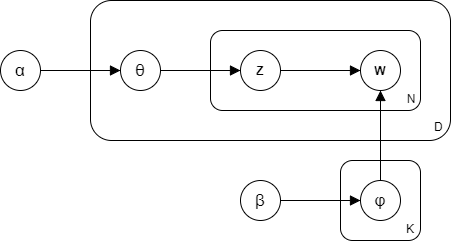
\includegraphics[width=7.5cm]{images/LDAModel}
\end{figure}\\
\hline
\end{tabular}
\end{adjustbox}
\captionof{figure}{{\itshape Model} LDA}
\end{table}

\indent
Berikut merupakan penjelasan dari bentuk-bentuk serta variabel-variabel yang terdapat pada Gambar 2.1.

\begin{enumerate}[nolistsep,leftmargin=0.5cm]
\item
Lingkaran \\
Lingkaran merupakan bentuk yang menunjukkan variabel-variabel yang akan digunakan selama proses LDA dilakukan.
\item
Tanda Panah \\
Tanda panah merupakan tanda yang menunjukkan ketergantungan antar 1 variabel dengan variabel yang lainnya.
\item
Kotak \\
Kotak merupakan bentuk yang menunjukkan bahwa bagian tersebut akan dilakukan perulangan ({\itshape looping}).
\end{enumerate}

\begin{table}[H]
\small
\centering
\caption{Deskripsi Model LDA}
\begin{adjustbox}{width=1\textwidth}
\begin{tabular}{| p {2 cm}| p {12 cm} |}
\hline
{\bfseries Variabel} & {\bfseries Deskripsi} \\ 
\hline
D & Jumlah dokumen \\
\hline
N & Jumlah semua kata yang ada dalam setiap dokumen \\
\hline
K & Jumlah topik \\
\hline
W & Jumlah setiap kata dalam setiap dokumen \\
\hline
Z & Topik untuk setiap kata dalam setiap dokumen \\
\hline
$\theta$ & Distribusi topik untuk dokumen tertentu \\
\hline
$\alpha$ & Bobot nilai untuk distribusi dokumen terhadap topik \\
\hline
$\beta$ & Bobot nilai untuk distribusi topik terhadap kata \\
\hline
$\varphi$ & Distribusi kata untuk topik tertentu \\
\hline
\end{tabular}
\end{adjustbox}
\end{table}

\indent
Berikut merupakan penjelasan proses dan {\itshape pseudocode} dari model {\itshape Latent Dirichlet Allocation} [10].

\begin{enumerate}[nolistsep,leftmargin=0.5cm]
\item
Menentukan jumlah topik yang akan digunakan sebagai jumlah label K yang unik dalam {\itshape corpus}.

\item
Mencari nilai {\itshape multinomial topic distributions} variabel $\varphi_k$ untuk setiap topik k, dari {\itshape Dirichlet prior} $\beta$.

\item	
Mencari {\itshape multinomial mixture distribution} $\theta^{(d)}$  terhadap semua topik K, untuk setiap dokumen d, dari {\itshape Dirichlet prior} $\alpha$.

\item	
Menentukan nilai z dengan menghitung {\itshape multinomial distribution} dari parameter $\theta^{(d)}$ dan tentukan juga nilai w dengan menghitung {\itshape multinomial distribution} dari parameter $\beta_z$ untuk sebanyak kata dalam setiap dokumen.
\end{enumerate}

\begin{table}[H]
\footnotesize
\begin{adjustbox}{width=1\textwidth}
\begin{tabular}{| p {14 cm}  |}
\hline
\makecell[l]{
\texttt{\small{1 For each topic k $\in$ \{1, ..., K\}:}}
\\\texttt{\small{2 \hspace{10mm}Generate $\varphi_{k}$ = (?$_{k,1}$, ..., $\varphi_{k,V}$)$^{T}\sim$ Dir(.$\mid\beta$)}}
\\\texttt{\small{3 \hspace{10mm}For each document d:}}
\\\texttt{\small{4 \hspace{10mm}\hspace{10mm}Generate $\theta^{(d)}$ = ($\theta _{l_{1}}$, ..., $\theta _{l_{M_{d}}}$)$^{T}\sim$ Dir(.$\mid\alpha$)}}
\\\texttt{\small{5 \hspace{10mm}\hspace{10mm}For each i in \{1, ..., N$_{d}$\}:}}
\\\texttt{\small{6 \hspace{10mm}\hspace{10mm}\hspace{10mm}Generate z$_{i}\in$\{$\lambda _{1}^{(d)}$, ..., $\lambda _{M_{d}}^{(d)}$\} $\sim$ Mult(.$\mid\theta^{(d)}$)}}
\\\texttt{\small{7 \hspace{10mm}\hspace{10mm}\hspace{10mm}Generate w$_{i}\in$\{1, ..., V\} $\sim$ Mult(.$\mid\varphi _{z_{i}}$)}}
} \\
\hline
\end{tabular}
\end{adjustbox}
\\[1.5pt]
\begin{center}\small{{\itshape {\bfseries Pseudocode}} 2.1 LDA}\end{center}
\end{table}

\subsection{{\itshape Labeled Latent Dirichlet Allocation}}
\indent
{\itshape Labeled Latent Dirichlet Allocation} (LLDA) merupakan model grafis probabilistik yang menggambarkan sebuah proses pembuatan dokumen berlabel. LLDA juga merupakan perluasan metode antara LDA (menggabungkan {\itshape supervision}) dan {\itshape Multinomial Naïve Bayes} (menggabungkan {\itshape mixture model}) [11]. Dalam pembelajaran mesin, LLDA merupakan metode yang masuk ke dalam kategori {\itshape supervised learning}. LLDA memodelkan sebuah dokumen dalam korpus sebagai campuran topik dan kata-kata yang dihasilkan oleh topik. Lalu, LLDA menyesuaikan antara topik laten dan label (korespondensi satu-satu), dimana label ini dapat dipelajari dan label tersebut merepresentasikan sebuah {\itshape class} [4].

\begin{table}[H]
\begin{adjustbox}{width=1\textwidth}
\begin{tabular}{| p {14 cm} |}
\hline
\begin{figure}[H]
	\centering
	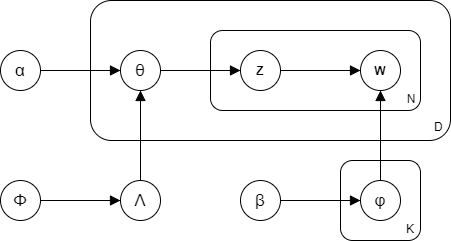
\includegraphics[width=7.5cm]{images/LLDAModel}
\end{figure}\\
\hline
\end{tabular}
\end{adjustbox}
\captionof{figure}{{\itshape Model} LLDA}
\end{table}

\indent
Gambar 2.2 merupakan gambar yang merepresentasikan model untuk LLDA. Fungsi dari setiap bentuk yang terdapat pada model LLDA sama seperti fungsi yang terdapat pada model LDA (Gambar 2.1). Berikut merupakan penjelasan variabel-variabel yang terdapat pada model LLDA.

\begin{table}[H]
\small
\centering
\caption{Deskripsi Model LLDA}
\begin{adjustbox}{width=1\textwidth}
\begin{tabular}{| p {2 cm}| p {12 cm} |}
\hline
{\bfseries Variabel} & {\bfseries Deskripsi} \\ 
\hline
$\Lambda$ & Sekumpulan biner yang menunjukan ada / tidaknya topik tersebut dalam sebuah dokumen \\
\hline
$\phi$ & Indikator ada / tidaknya topik-topik untuk sebuah dokumen \\
\hline
\end{tabular}
\end{adjustbox}
\end{table}

\indent
Berikut merupakan penjelasan proses dan {\itshape pseudocode} dari model {\itshape Labeled Latent Dirichlet Allocation} (Gambar 2.2) [9].

\newcounter{numberedCntDA}
\begin{enumerate}[nolistsep,leftmargin=0.5cm]
\item
Menentukan jumlah topik yang akan digunakan sebagai jumlah label K yang unik dalam \textit{corpus}.

\item
Mencari nilai \textit{multinomial topic distributions} variabel $\varphi _{k}$ untuk setiap topik k, dari \textit{Dirichlet prior} $\beta$.

\item 
Dalam model LDA, langkah selanjutnya yang dilakukan adalah mencari \textit{multinomial mixture distribution} $\theta ^{(d)} $terhadap semua topik K, untuk setiap dokumen \textit{d}, dari \textit{Dirichlet prior} $\alpha$. Dalam model LLDA, terdapat batasan untuk nilai $\theta ^{(d)}$, dimana nilai tersebut harus didefinisikan hanya terhadap topik yang sesuai dengan labelnya $\Lambda ^{(d)}$. Jadi langkah selanjutnya yang harus dilakukan adalah mencari nilai $\Lambda ^{(d)}$ dengan melihat label dari setiap dokumen menggunakan \textit{Bernoulli coin toss} untuk setiap topik k, dengan \textit{labeling prior probability} $\Phi _{k}$.

\item 
Menentukan vektor dari label setiap dokumen menjadi $\lambda ^{(d)}= \lbrace k\mid\Lambda _{k}^{(d)}=1\rbrace $.

\item 
Nilai $\lambda ^{(d)}$ pada langkah 4 digunakan untuk mendefinisikan proyeksi matriks dari label setiap dokumen secara spesifik dengan persamaan $L^{(d)}= M_{d}$ x K untuk setiap dokumen d, dimana $M_{d}= \mid \lambda ^{(d)}\mid$. Di bawah 
ini merupakan \textit{rule} untuk menentukan nilai $L^{(d)}$ dengan baris $i \in \lbrace 1, \ldots ,M_{d}\rbrace $ dan kolom $j \in \lbrace 1, \ldots ,K\rbrace $.
\setcounter{numberedCntDA}{\theenumi}

\begin{table}[H]
\small
\centering
\begin{adjustbox}{width=1\textwidth}
\begin{tabular}{| p {14 cm} |}
\hline
$$
  L_{ij}^{(d)}=\begin{cases}
    1, & \text{if $\lambda_{i}^{(d)}= j$}.\\
    0, & \text{if $\lambda _{i}^{(d)}\ne j$}.
  \end{cases}
$$
\\
\hline
\end{tabular}
\end{adjustbox}
\end{table}

\begin{tabbing}[H]
\phantom{$D_{n50}\ $}\= \kill
\small{\hspace{60mm}$\lambda ^{(d)}$ = Vektor Label}\\
\end{tabbing}

Contoh: misalkan \textit{K} = 4 dan dokumen d memiliki label yang diberikan oleh $\Lambda ^{(d)}= \lbrace 1, 0, 0, 1\rbrace $. Nilai $\Lambda ^{(d)}$ menghasilkan nilai $\lambda ^{(d)}= \lbrace 1, 4\rbrace $. Setelah mendapat nilai dari $\lambda ^{(d)}$, maka nilai $L^{(d)}$ akan menjadi :

\begin{table}[H]
\footnotesize
\centering
\begin{adjustbox}{width=1\textwidth}
\begin{tabular}{| p {14 cm} |}
\hline
$$
\begin{pmatrix} 
1 & 0 & 0 & 0 \\
0 & 0 & 0 & 1 
\end{pmatrix}
$$\\
\hline
\end{tabular}
\end{adjustbox}
\end{table}
\end{enumerate}

\begin{enumerate}
\setcounter{enumi}{\thenumberedCntDA}
\item 
Gunakan nilai dari matriks $L^{(d)}$ untuk memproyeksikan vektor dengan parameter \textit{Dirichlet topic prior} \textit{$\alpha$}, dimana hasil proyeksi ini akan menghasilkan nilai $\alpha ^{(d)}$ (vektor dengan dimensi yang lebih kecil) dengan banyak nilai $M_{d}= \sum_{k=1}^{K}{\Lambda _{k}^{(d)}}$.
\setcounter{numberedCntDA}{\theenumi}
\end{enumerate}

\begin{table}[H]
\small
\centering
\begin{adjustbox}{width=1\textwidth}
\begin{tabular}{| p {14 cm} |}
\hline
$$
\alpha ^{(d)}= L^{(d)} x \alpha = (\alpha _{\lambda _{i}^{(d)}}, \ldots ,\alpha _{\lambda _{M_{d}}^{(d)}})^{T}
$$\\
\hline
\end{tabular}
\end{adjustbox}
\end{table}

\begin{tabbing}[H]
\phantom{$D_{n50}\ $}\= \kill
\small{\hspace{60mm}$L^{(d)}$ = Proyeksi Matriks Label}
\end{tabbing}

\begin{enumerate}
\setcounter{enumi}{\thenumberedCntDA}
\item 
Menentukan nilai $\theta ^{(d)}$ dengan menghitung \textit{Dirichlet distribution} dari parameter $\alpha ^{(d)}$.

\item 
Menentukan nilai z dengan menghitung \textit{multinomial distribution} dari parameter $\theta ^{(d)}$ dan tentukan juga nilai w dengan menghitung \textit{multinomial distribution} dari parameter $\beta _{z}$ untuk sebanyak kata dalam setiap dokumen.

\setcounter{numberedCntDA}{\theenumi}
\end{enumerate}

\begin{table}[H]
\footnotesize
\begin{adjustbox}{width=1\textwidth}
\begin{tabular}{| p {14 cm}  |}
\hline
\makecell[l]{
\texttt{\small{1  For each topic k $\in$ \{1, ..., K\}:}}
\\\texttt{\small{2 \hspace{10mm} Generate $\varphi _{k}$ = ($\varphi_{k,1}$, ..., $\varphi_{k,V}$)$^{T}\sim$ Dir(.$\mid\beta$)}}
\\\texttt{\small{3 \hspace{10mm} For each document d: }}
\\\texttt{\small{4 \hspace{10mm}\hspace{10mm} For each topic k $\in$ \{1, ..., K\}:}}
\\\texttt{\small{5 \hspace{10mm}\hspace{10mm}\hspace{10mm} Generate $\Lambda^{(d)}$ k $\in$ \{0,1\} $\sim$ Bernoulli(.$\mid\phi_{k}$)}}
\\\texttt{\small{6 \hspace{10mm}\hspace{10mm}\hspace{10mm} Generate $\alpha^{(d)}$ = L$^{(d)}$ x $\alpha$}}
\\\texttt{\small{7 \hspace{10mm}\hspace{10mm}\hspace{10mm} Generate $\theta ^{(d)}$$^{ }$= ($\theta _{l_{1}}$, ..., $\theta _{l_{M_{d}}}$)$^{T}\sim$ Dir(.|$\alpha^{(d)}$)}}
\\\texttt{\small{8 \hspace{10mm}\hspace{10mm} For each i in \{1, ..., N$_{d}$\}:}}
\\\texttt{\small{9 \hspace{10mm}\hspace{10mm}\hspace{10mm} Generate z$_{i}\in$ \{$\lambda _{1}^{(d)}$, ..., $\lambda _{M_{d}}^{(d)}$\} $\sim$ Mult(.$\mid\theta^{(d)}$)}}
\\\texttt{\small{10 \hspace{10mm}\hspace{10mm}\hspace{10mm}Generate w$_{i}\in$ \{1, ..., V\} $\sim$ Mult(.$\mid\varphi _{z_{i}}$)}}
} \\
\hline
\end{tabular}
\end{adjustbox}
\\[1.5pt]
\begin{center}\small{{\itshape {\bfseries Pseudocode}} 2.2 LLDA}\end{center}
\end{table}

\subsection{{\itshape Simplified Labeled Latent Dirichlet Allocation Classifier} (SLLDA-C)}
\indent
{{\itshape Simplified Labeled Latent Dirichlet Allocation Classifier} (SLLDA-C) merupakan metode {\itshape Labeled Latent Dirichlet Allocation} yang prosesnya dibuat menjadi lebih sederhana. Di bawah ini merupakan langkah proses dari SLLDA-C [4].

\begin{enumerate}[nolistsep,leftmargin=0.5cm]
\item
Dapatkan nilai $\Lambda$ dari data {\itshape training}. Nilai $\Lambda$ bisa didapat langsung dari data {\itshape training}, karena setiap dokumen dalam {\itshape corpus} pasti memiliki 1 label.
\item
Lakukan pembelajaran ({\itshape learning}) terhadap data {\itshape training} untuk mendapatkan nilai $\varphi$ menggunakan {\itshape Collapsed Gibbs Sampling} dengan menggunakan nilai $\alpha$ dan $\beta$ yang telah ditentukan serta nilai $\Lambda$ yang telah dipelajari terlebih dahulu pada langkah 1.
\item
Setelah nilai $\varphi$ dipelajari dari data {\itshape training}, ekstrak 20\% kata dengan probabilitas tertinggi untuk setiap topik dari $\varphi$.
\item
Tetapkan label k ke dokumen jika dokumen tersebut memiliki kata-kata yang paling berkaitan dengan topik k.
\end{enumerate}

\subsection{{\itshape Gibbs Sampling}}
\indent
{\itshape Gibbs Sampling} merupakan algoritma {\itshape Markov Chain Monte Carlo} (MCMC) untuk memperoleh serangkaian pengamatan berdasarkan distribusi {\itshape multivariate} tertentu. Algoritma ini digunakan ketika pengambilan {\itshape sample} secara langsung sulit untuk dilakukan. Dalam LDA, {\itshape Gibbs Sampling} digunakan untuk menyederhanakan persamaan matematika yang berfungsi untuk melakukan pembelajaran ({\itshape learning}) serta pengambilan keputusan ({\itshape inference}) [12]. Di bawah ini merupakan rumus dari {\itshape Gibbs Sampling}.

\definecolor{Gray}{gray}{0.85}
\begin{table}[H]
\small
\centering
\begin{adjustbox}{width=1\textwidth}
\begin{tabular}{| p {14 cm} |}
\hline
\rowcolor{Gray}
\begin{equation}
\begin{split}
p(z_{i}=j \mid z_{-i}^{(d)}, w^{(d)}) \propto p(z_{i}=j, w_{i}=t \mid z_{-i}^{(d)}, w_{-i}^{(d)})\\
 = E(\theta _{dj}).E(\phi _{jt})
\end{split}
\end{equation}\\
\hline
\end{tabular}
\end{adjustbox}
\end{table}

\definecolor{Gray}{gray}{0.85}
\begin{table}[H]
\small
\centering
\begin{adjustbox}{width=1\textwidth}
\begin{tabular}{| p {14 cm} |}
\hline
\rowcolor{Gray}
\begin{equation}
E(\varphi _{jt})= \dfrac{n_{-i, j}^{(t)}+ \beta_{t}}{W}
\end{equation}\\
\hline
\end{tabular}
\end{adjustbox}
\end{table}

\begin{tabbing}[H]
\phantom{$D_{n50}\ $}\= \kill
\small{\hspace{35mm}$\beta_t$ = Nilai Beta untuk Kata ke-t}\\
\small{\hspace{35mm}$n_{-i,j}^{(t)}$ = Jumlah Kata t pada Topik j Dikurangi 1}
\end{tabbing}

\definecolor{Gray}{gray}{0.85}
\begin{table}[H]
\small
\centering
\begin{adjustbox}{width=1\textwidth}
\begin{tabular}{| p {14 cm} |}
\hline
\rowcolor{Gray}
\begin{equation}
E(\theta _{dj})= \dfrac{n_{-i, j}^{(d)}+ \alpha_{j}^{(d)}}{T}
\end{equation}\\
\hline
\end{tabular}
\end{adjustbox}
\end{table}

\begin{tabbing}[H]
\phantom{$D_{n50}\ $}\= \kill
\small{\hspace{30mm}$\alpha_j^{(d)}$ = Nilai Alpha untuk Topik ke-j Pada Dokumen d}\\
\small{\hspace{30mm}$n_{-i,j}^{(d)}$ = Jumlah Kata di Dokumen d Pada Topik j Dikurangi 1}
\end{tabbing}

\definecolor{Gray}{gray}{0.85}
\begin{table}[H]
\small
\centering
\begin{adjustbox}{width=1\textwidth}
\begin{tabular}{| p {14 cm} |}
\hline
\rowcolor{Gray}
\begin{equation}
W= \sum_{t=1}^{V}{n_{-i, j}^{(t)}} + \sum_{l=1}^{V}{\beta _{l}}
\end{equation}\\
\hline
\end{tabular}
\end{adjustbox}
\end{table}

\begin{tabbing}[H]
\phantom{$D_{n50}\ $}\= \kill
\small{\hspace{35mm}$\beta_l$ = Nilai Beta untuk Kata ke-l}\\
\small{\hspace{35mm}$n_{-i,j}^{(t)}$ = Jumlah Kata t pada Topik j Dikurangi 1}
\end{tabbing}

\definecolor{Gray}{gray}{0.85}
\begin{table}[H]
\small
\centering
\begin{adjustbox}{width=1\textwidth}
\begin{tabular}{| p {14 cm} |}
\hline
\rowcolor{Gray}
\begin{equation}
T=\sum_{k?\lambda ^{(d)}}{n_{-i, k}^{(d)}}+ \sum_{k=1}^{M_{d}}{\alpha_{k}^{(d)}}
\end{equation}\\
\hline
\end{tabular}
\end{adjustbox}
\end{table}

\begin{tabbing}[H]
\phantom{$D_{n50}\ $}\= \kill
\small{\hspace{30mm}$\alpha_j^{(d)}$ = Nilai Alpha untuk Topik ke-j Pada Dokumen d}\\
\small{\hspace{30mm}$n_{-i,j}^{(d)}$ = Jumlah Kata di Dokumen d Pada Topik j Dikurangi 1}
\end{tabbing}

\indent
Berikut merupakan penjelasan proses dan {\itshape pseudocode} dari algoritma {\itshape Gibbs Sampling} [13].

\begin{enumerate}[nolistsep,leftmargin=0.5cm]
\item
Pilih kata beserta topik untuk dilakukan pembelajaran.
\item
Berasumsi bahwa kata pada topik tersebut belum pernah masuk sebelumnya. Untuk melakukan hal tersebut maka lakukan pengurangan ({\itshape decrement}) terhadap jumlah dokumen terhadap topik dan topik terhadap kata.
\item
Hitung nilai probabilitas dari kata tersebut terhadap jumlah topik yang ada pada setiap dokumen.
\item
Tetapkan kata tersebut dengan topik yang memiliki probabilitas tertinggi.
\item
Lakukan penambahan ({\itshape increment}) untuk jumlah dokumen terhadap topik dan jumlah topik terhadap kata.
\item
Lakukan langkah 1-5 hingga semua kata telah dilakukan pembelajaran.
\item
Lakukan langkah 1-6 hingga iterasi {\itshape Gibbs Sampling} selesai.
\end{enumerate}

\begin{table}[H]
\footnotesize
\begin{adjustbox}{width=1\textwidth}
\begin{tabular}{| p {14 cm}  |}
\hline
\makecell[l]{
\texttt{\small{1 For each iteration:}}
\\\texttt{\small{2 \hspace{10mm}For each document d:}}
\\\texttt{\small{3 \hspace{10mm}\hspace{10mm}For each i in \{0, ..., N-1\}:}}
\\\texttt{\small{4 \hspace{10mm}\hspace{10mm}\hspace{10mm}word $<$- w$[$i$]$}}
\\\texttt{\small{5 \hspace{10mm}\hspace{10mm}\hspace{10mm}topic $<$- z$[$i$]$}}
\\\texttt{\small{6 \hspace{10mm}\hspace{10mm}\hspace{10mm}$n_{d, topic}$ -= 1}}
\\\texttt{\small{7 \hspace{10mm}\hspace{10mm}\hspace{10mm}$n_{word, topic}$ -= 1}}
\\\texttt{\small{8 \hspace{10mm}\hspace{10mm}\hspace{10mm}For each k in \{0, ..., $M_{d}-1$\}:}}
\\\texttt{\small{9 \hspace{10mm}\hspace{10mm}\hspace{10mm}\hspace{10mm}$p(z=k .)= E(\theta _{dj}).E(\varphi _{jt})$}}
\\\texttt{\small{10 \hspace{10mm}\hspace{10mm}\hspace{10mm}topic $<$- sample dari $p(z .)$}}
\\\texttt{\small{11 \hspace{10mm}\hspace{10mm}\hspace{10mm}$n_{d, topic}$ += 1}}
\\\texttt{\small{12 \hspace{10mm}\hspace{10mm}\hspace{10mm}$n_{word, topic}$ += 1}}
} \\
\hline
\end{tabular}
\end{adjustbox}
\\[1.5pt]
\begin{center}\small{{\itshape {\bfseries Pseudocode}} 2.3 {\itshape Gibbs Sampling}}\end{center}
\end{table}

\subsection{{\itshape F-Measure}}
\indent
Tingkat akurasi merupakan salah satu aspek yang penting dalam hal kategorisasi. Suatu sistem kategorisasi dapat dikatakan baik, jika hasil kategori yang dihasilkan oleh sistem memiliki tingkat akurasi yang tinggi. Untuk mengukur tingkat akurasi dari sistem kategorisasi, terdapat beberapa metode perhitungan untuk menghitung seberapa akurat hasil kategori yang dihasilkan oleh sistem. Metode perhitungan tersebut di antaranya menggunakan {\itshape precision} dan {\itshape recall} [4]. Di bawah ini merupakan rumus-rumus untuk mengukur nilai akurasi.

\begin{enumerate}[nolistsep,leftmargin=0.5cm]
\item 
{\itshape Precision}

\definecolor{Gray}{gray}{0.85}
\begin{table}[H]
\small
\centering
\begin{adjustbox}{width=1\textwidth}
\begin{tabular}{| p {14 cm} |}
\hline
\rowcolor{Gray}
\begin{equation}
P_i = \dfrac{TP_i}{TP_i + FP_i}
\end{equation}\\
\hline
\end{tabular}
\end{adjustbox}
\end{table}

\begin{tabbing}[H]
\phantom{$D_{n50}\ $}\= \kill
\small{\hspace{60mm}$P_i$ = Precision}\\
\small{\hspace{60mm}$TP_i$ = True Positive}\\
\small{\hspace{60mm}$FP_i$ = False Positive}
\end{tabbing}

\item
{\itshape Recall}

\definecolor{Gray}{gray}{0.85}
\begin{table}[H]
\small
\centering
\begin{adjustbox}{width=1\textwidth}
\begin{tabular}{| p {14 cm} |}
\hline
\rowcolor{Gray}
\begin{equation}
R_i = \dfrac{TP_i}{TP_i + FN_i}
\end{equation}\\
\hline
\end{tabular}
\end{adjustbox}
\end{table}

\begin{tabbing}[H]
\phantom{$D_{n50}\ $}\= \kill
\small{\hspace{60mm}$R_i$ = Recall}\\
\small{\hspace{60mm}$TP_i$ = True Positive}\\
\small{\hspace{60mm}$FN_i$ = False Negative}
\end{tabbing}

\item
{\itshape F-Measure}

\definecolor{Gray}{gray}{0.85}
\begin{table}[H]
\small
\centering
\begin{adjustbox}{width=1\textwidth}
\begin{tabular}{| p {14 cm} |}
\hline
\rowcolor{Gray}
\begin{equation}
F-Measure = \dfrac{2 * (P * R)}{P + R}
\end{equation}\\
\hline
\end{tabular}
\end{adjustbox}
\end{table}

\begin{tabbing}[H]
\phantom{$D_{n50}\ $}\= \kill
\small{\hspace{65mm}$P$ = Precision}\\
\small{\hspace{65mm}$R$ = Recall}
\end{tabbing}

\end{enumerate}

\indent
Berikut merupakan penjelasan mengenai {\itshape true positive}, {\itshape false negative}, dan {\itshape false positive}.

\begin{enumerate}[nolistsep,leftmargin=0.5cm]
\item
{\itshape True Positive} merupakan nilai pada baris dan kolom yang sama.
\item
{\itshape False Negative} merupakan penjumlahan nilai pada baris yang sesuai (tanpa mengikutsertakan nilai {\itshape true positive}).
\item
{\itshape False Positive} merupakan penjumlahan nilai pada kolom yang sesuai (tanpa mengikutsertakan nilai {\itshape true positive}).
\end{enumerate}

\indent
Sebagai contoh, di bawah ini merupakan hasil klasifikasi dari tiga kelas (A, B, dan C) yang akan digunakan untuk mencari nilai {\itshape F-Measure}.

\begin{table}[H]
\small
\centering
\caption{{\itshape Confusion Matrix}}
\begin{adjustbox}{width=1\textwidth}
\begin{tabular}{| p {3.5 cm} | p {3.5 cm} | p {3.5 cm} | p {3.5 cm} |}
\hline
 & {\bfseries A} & {\bfseries B} & {\bfseries C} \\
\hline
{\bfseries A} & 8 & 2 & 1 \\
\hline
{\bfseries B} & 3 & 7 & 0 \\
\hline
{\bfseries C} & 1 & 0 & 5 \\
\hline
\end{tabular}
\end{adjustbox}
\end{table}

\indent
Untuk melakukan pencarian nilai {\itshape F-Measure}, langkah awal yang harus dilakukan adalah mencari nilai {\itshape true positive}, {\itshape false negative}, dan {\itshape false positive} terlebih dahulu. Setelah ketiga nilai tersebut didapatkan, lakukan perhitungan untuk mencari nilai {\itshape precision} dan {\itshape recall}.

\begin{table}[H]
\small
\centering
\caption{Contoh Hasil Perhitungan {\itshape F-Measure}}
\begin{adjustbox}{width=1\textwidth}
\begin{tabular}{| p {3.5 cm} | p {3.5 cm} | p {3.5 cm} | p {3.5 cm} |}
\hline
 & {\bfseries A} & {\bfseries B} & {\bfseries C} \\
\hline
{\bfseries TP} & 8 & 7 & 5 \\
\hline
{\bfseries FN} & 3 & 3 & 1 \\
\hline
{\bfseries FP} & 4 & 2 & 1 \\
\hline
{\bfseries Precision} & 0.666666667 & 0.777777778 & 0.833333333 \\
\hline
{\bfseries Recal}l & 0.727272727 & 0.7 & 0.833333333 \\
\hline
\end{tabular}
\end{adjustbox}
\end{table}

\begin{table}[H]
\small
\centering
\begin{adjustbox}{width=1\textwidth}
\begin{tabular}{| p {3.5 cm} | p {3.5 cm} | p {3.5 cm} | p {3.5 cm} |}
\hline
{\bfseries F-Measure} & 0.695652174 & 0.736842105 & 0.833333333 \\
\hline
\end{tabular}
\end{adjustbox}
\end{table}

\section{Tinjauan Studi}
\indent 
Tinjauan studi merupakan bagian yang menjelaskan sumber-sumber pembelajaran yang digunakan selama melakukan peneltian.

\subsection{{\itshape State of the Art}}
\indent
Untuk mendukung penelitian yang dilakukan, dibutuhkan beberapa jurnal yang terkait dengan metode maupun topik penelitian. Jurnal-jurnal ini digunakan sebagai tinjauan penulis dalam melakukan penelitian. Tabel 2.16 merupakan tabel yang merepresentasikan jurnal-jurnal yang digunakan sebagai tinjauan studi.

\begin{table}[H]
\small
\centering
\caption{{\itshape State of the Art}}
\begin{adjustbox}{width=1\textwidth}
\begin{tabular}{| p {2 cm} | p {4 cm}| p {1 cm} | p {4 cm} | p {2 cm} |}
\hline
{\bfseries Peneliti} & {\bfseries Judul} & {\bfseries Tahun} & {\bfseries Masalah} & {\bfseries Metode} \\ 
\hline
Yiqi Bai, Jie Wang & News Classifications with Labeled LDA & 2015 & Melakukan klasifikasi terhadap berita dengan melakukan modifikasi terhadap Labeled LDA untuk meningkatkan tingkat akurasi & LLDA-C, SLLDA-C, SVM \\ 
\hline
Daniel Ramage, David Hall, Ramesh Nallapati, Christopher D. Manning & Labeled LDA: A supervised topic model for credit attribution in multi labeled-corpora & 2009 &Mencoba menyelesaikan permasalahan multi-tag pada kasus credit attribution dengan menggunakan metode pengembangan dari LDA (LLDA). & LLDA, SVM \\ 
\hline
Ge Song, Yunming Ye, Xiaolin Du, Xiaohui Huang, Shifu Bie & Short Text Classification: A Survey & 2014 & Melakukan klasifikasi terhadap teks yang pendek & LSA, pLSA, LDA \\ 
\hline
\end{tabular}
\end{adjustbox}
\end{table}

\section{Tinjauan Objek}
\indent
Berikut merupakan objek-objek yang akan digunakan dalam penelitian sistem kategorisasi dokumen.

\begin{enumerate}[nolistsep,leftmargin=0.5cm]
\item
Abstraksi \\
Abstraksi merupakan uraian singkat tetapi lengkap yang berisi judul, permasalahan pendekatan terhadap masalah landsan teoritik yang digunakan, hasil temuan, dan rekomendasi. Fungsi abstrak adalah memberikan gambaran kepada pembaca mengenai isi laporan yang akan dibacanya. Isi abstrak meliputi judul penelitian, rumusan masalah penelitian, metode penelitian, teknik dan pengumpulan data penelitian serta hasil dan kesimpulan peneltian yang telah dibuat
\item
Jurnal Penelitian \\
Jurnal penelitian merupakan sebuah laporan peneliti tentang hasil penelitian yang telah dilakukan secara ilmiah atau merupakan kesimpulan dari penelitian skripsi yang telah dilakukan. Pada dasarnya, sebagian besar jurnal penelitian dapat dipertanggungjawabkan keilmiahannya tergantung dari metode yang dipakai dalam pembuatan dan penyusunan laporan jurnal penelitian. Biasanya laporan jurnal penelitian dimasukkan dalam terbitan kumpulan jurnal bersama-sama dengan laporan peneliti lain. Contoh sumber untuk mendapat jurnal penelitian diantaranya dapat dilihat pada website IEEE, ACM, dan {\itshape Research Gate}.
\end{enumerate}
\newpage